\section{Architektur}
\label{sec:arch}
Grundsätzlich lassen sich zwei unterschiedliche Architekturansätze im Bereich Data Streaming unterscheiden:

\begin{description}
\item [Lambda Architektur:] Benannt nach dem griechischen $\lambda$ zeichnet sich dieser Ansatz dadurch aus, dass die Streaming Daten zweigleisig verarbeitet werden. Zum einen wird der Datenstrom direkt in einen häufig auf In-Memory Technologie basierenden \textit{Speed Layer} geleitet, der diese in Echtzeit verarbeitet und dem \textit{Serving Layer} zur Verfügung stellt. Da Streams per Definition unendlich und der Speed Layer teuer und physikalisch endlich ist, wird der Stream von \textit{Ingestion Layer} parallel in den \textit{Batch Layer} geleitet. Dieser speichert zunächst die Daten persistent und startet nach einem fest definierten Intervall einen Batch-Job um die bis dahin angelaufenen Daten zu verarbeiten und zum Serving Layer zu übertragen. Es ist also die nicht zu unterschätzende  Verantwortung des Serving Layers, die aggregierten Bestandsdaten aus dem Batch Layer mit den Echtzeitdaten des Speed Layers, die noch nicht vom Batch Layer verarbeitet worden sind, abzumischen.\autocite{lambda-architecture} \autocite{jaxkappa} 

\begin{figure}[h]
	\centering
	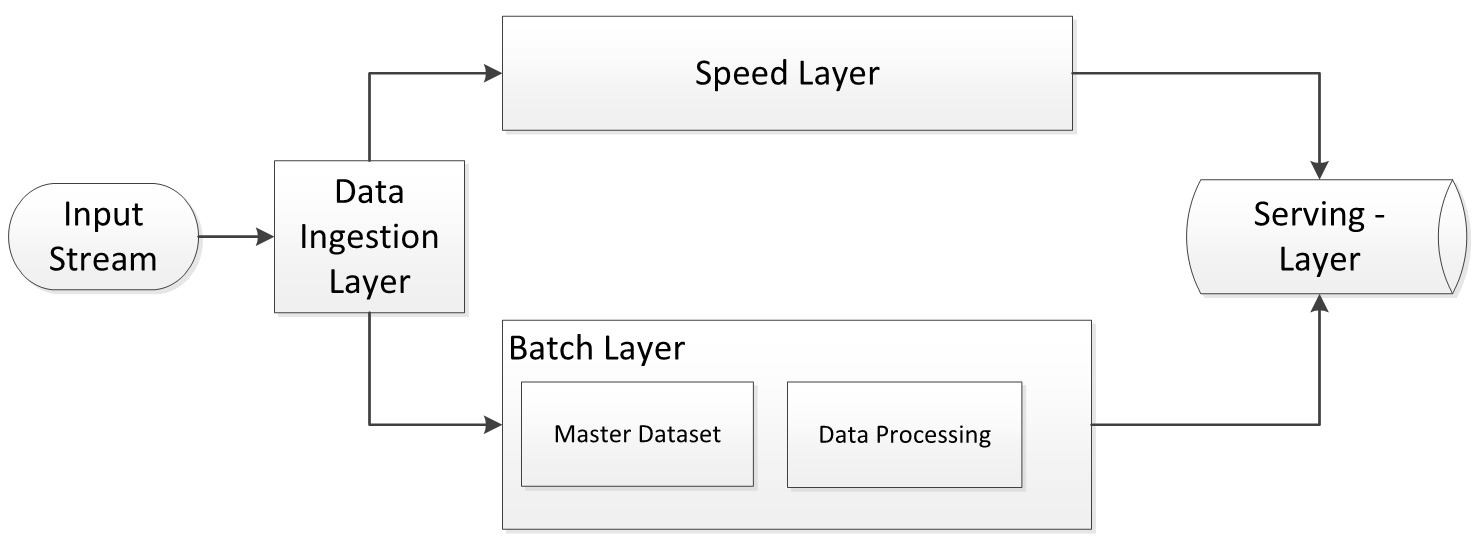
\includegraphics[width=10cm]{berle_lambda-architektur_3.jpg}
	\caption[Schema der $\lambda$ Architektur]{Schema der $\lambda$ Architektur\autocite{jaxkappa}}
	\label{fig:KafkaArchitecture}
\end{figure}


\item [Kappa Architektur:] Dieser von Confluent Mitgründer und CEO Jay Kreps entworfene Ansatz verzichtet auf eine Batch-Verarbeitung und kommt somit mit lediglich mit \textit{Ingestion-}, \textit{Speed-} und \textit{Serving-Layer} aus. Damit spart man sich Entwicklung und Betrieb von zwei separaten Schichten und das aufwändige Abmischen von Batch-Daten mit Live-Daten im \textit{Serving-Layer}. Voraussetzung ist allerdings, dass der \textit{Ingestion-Layer} nicht nur Daten volatil durchreicht sondern vielmehr als \textbf{Puffer} die Rohdaten persistent im \textit{Master-Dataset} vorhält, um im Falle einer neuen, noch nicht vorberechneten Anfrage oder Änderung im \textit{Speed-Layer} die Rohdaten erneut bereit zu stellen. Um ein korrektes Replay der Nachrichten sicherzustellen beruht der Puffer auf einem kanonisches Log, in dem lediglich Nachrichten unverändert hinzugefügt, aber bereits gespeicherte Nachrichten nicht mehr verändert oder in ihrer Reihenfolge verschoben werden können. Um gleichzeitig Nähe als auch Abgrenzung zur $\lambda$ Architektur zu veranschaulichen wurde dieser Ansatz nach dem griechischen $\kappa$ benannt.\autocite{Kappa-Architektur} {Kappa-Architektur2}

\begin{figure}[h]
	\centering
	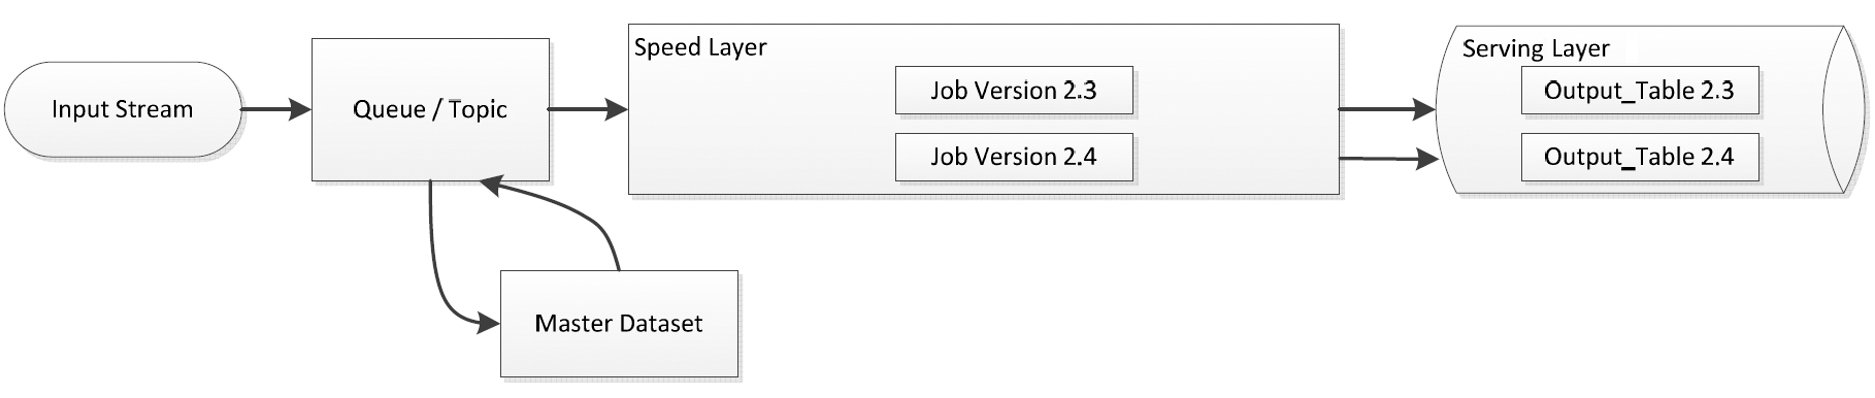
\includegraphics[width=10cm]{berle_lambda-architektur_4.jpg}
	\caption[Schema der $\kappa$ Architektur]{Schema der $\kappa$ Architektur\autocite{jaxkappa}}
	\label{fig:KappaArchitecture}
\end{figure}

\end{description}

Der erste Lösungsentwurf für unser Problem orientiert sich an der Lambda Architektur. Weil die von uns gewählte Datenquelle kein Stream sondern ein statisches, online abrufbares Datenset ist, sieht unser Lösungsansatz vor, mittels eines Kafka Producers \textbf{(1)} die Online-Daten zu laden und sukzessive in einen Kafka Topic zu schreiben, um somit eine Art Pseudo-Stream zu imitieren. Da das Web-API ohnehin \textit{Paging} über das Datenset erlaubt sollte die Implementierung nicht sonderlich kompliziert sein.

In Schritt \textbf{(2)} sammelt ein Consumer zeitgesteuert die Nachrichten des Kafka Topics ein und schreibt die Daten per SQL \code{INSERT} \footnote{Um die IO-Last der Datenbankverbindung gering zu halten sollte die Daten per BULK-INSERT erfolgen} in eine relationale Datenbanktabelle. Auf dieser Tabelle horcht ein \code{AFTER INSERT TRIGGER} \textbf{(3)}, der, sobald Daten in die Tabelle geschrieben wird, eine \code{FUNCTION} bzw. \code{STORED PROCEDURE} aufruft um Aggregate über die neuen Datensätze zu berechnen und in einer separaten Tabelle abzuspeichern bzw. mit bereits bestehenden Aggregaten zu verrechnen. Danach kann die Tabelle mit den Rohdaten theoretisch geleert werden, spätestens jedoch sobald der verfügbare Speicherplatz zu neige geht\footnote{Alternativ könnte man einen \code{INSTEAD OF TRIGGER} benutzen und ausschließlich Aggregate permanent zu speichern}.

Parallel dazu konsumiert ein in Zeppelin- oder Jupyter-Notebook eingebetteter Consumer\footnote{Apache Spark liefert bereits eine Kafka-Consumer Bibliothek} die Rohdaten aus dem gleichen Topic \textbf{(4)}.

\begin{figure}[h] %http://spark.apache.org/docs/latest/streaming-kafka-0-10-integration.html
	\centering
	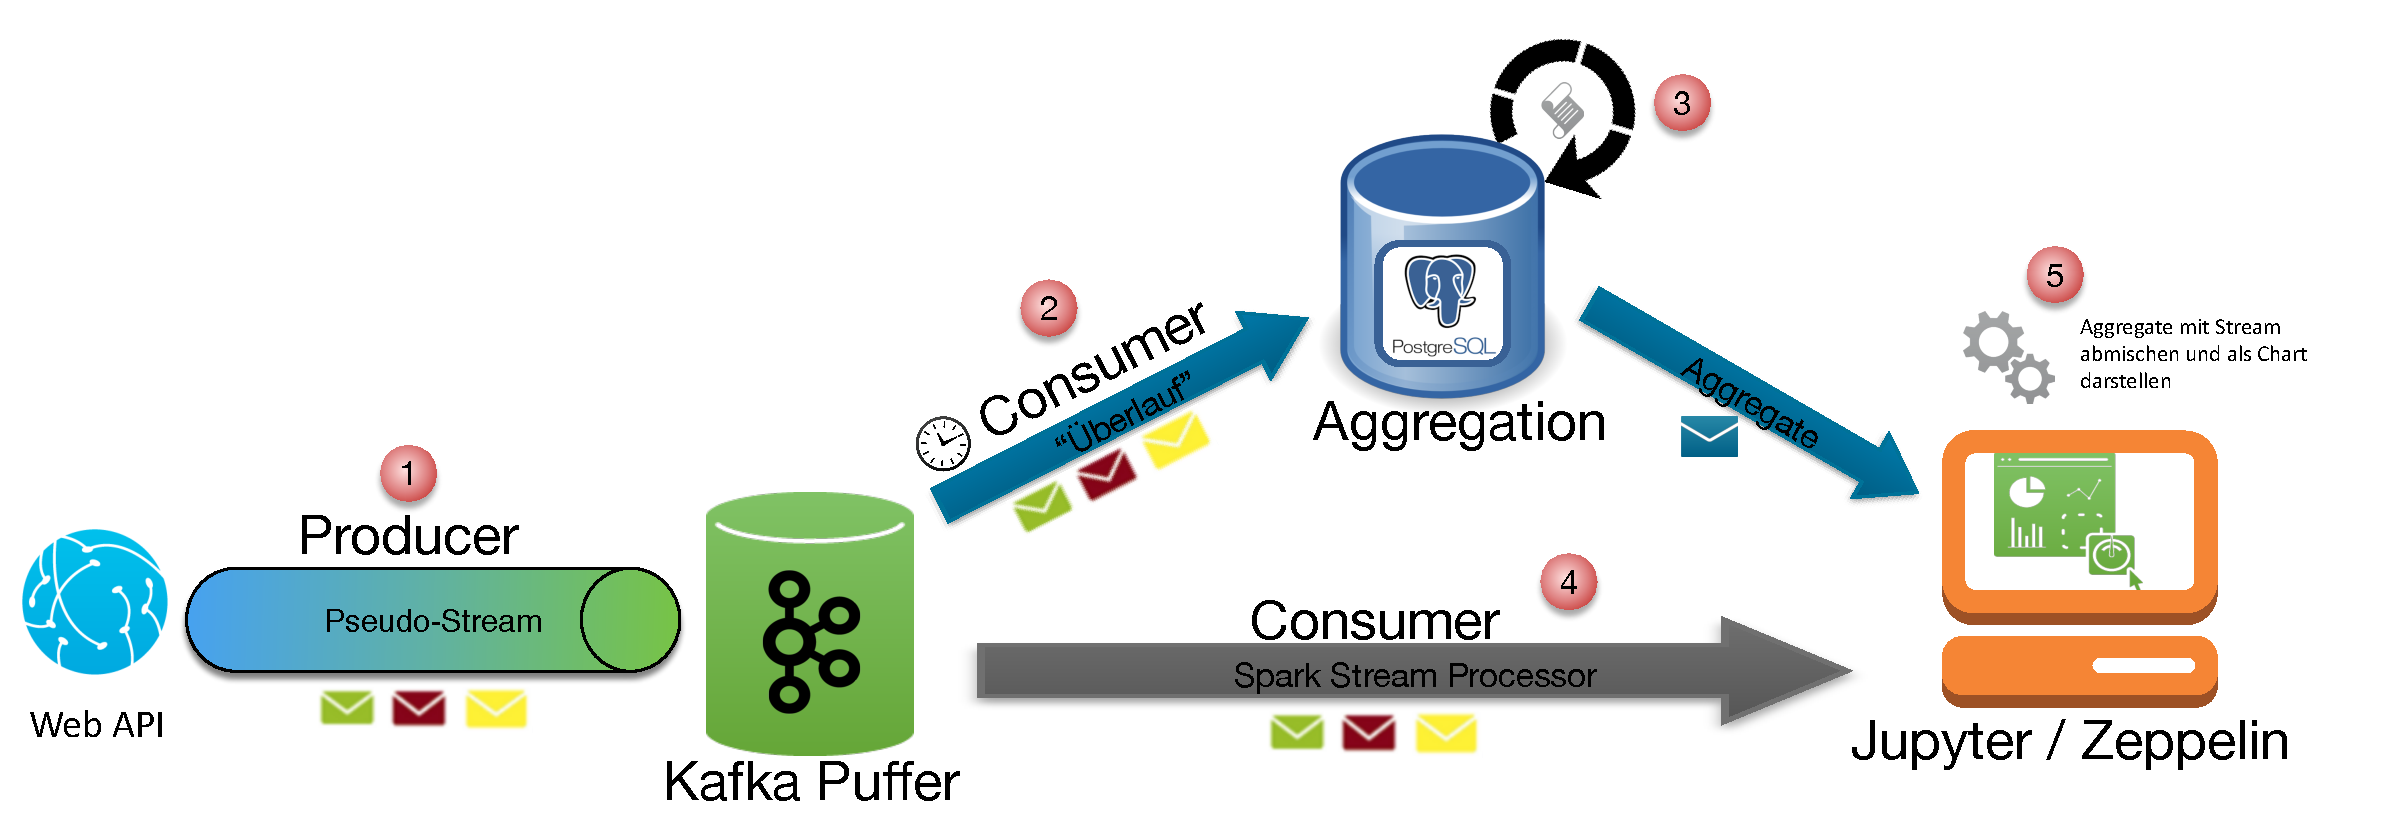
\includegraphics[width=\linewidth]{Overview_lampda.pdf}
	\caption[Lösungsentwurf nach $\lambda$]{Lösungsentwurf nach $\lambda$}
	\label{fig:OurLampdaArchitecture}
\end{figure}

Somit wären im Auswertungs-Dashboard \textbf{(5)} sowohl Charting auf Live-Daten als auch über aggregierte Bestandsdaten aus PostgreSQL, die ggf. aus Speicherplatzgründen gar nicht mehr in Kafka vorgehalten werden können, möglich. Der Serving Layer würde in diesem Fall in die Auswertungskomponente fallen.


Da allerdings mit diesem Ansatz die bereits erörterten Nachteile der Lambda Architektur einhergehen und wir in unserem Beispiel keinen unendlichen Stream sondern eine endliche Datenmenge haben, die ganzheitlich in den Kafka-Puffer passt, haben wir den Lösungsentwurf überarbeitet und an die einfachere Kappa-Architektur angeglichen.

\begin{figure}[h] %http://spark.apache.org/docs/latest/streaming-kafka-0-10-integration.html
	\centering
	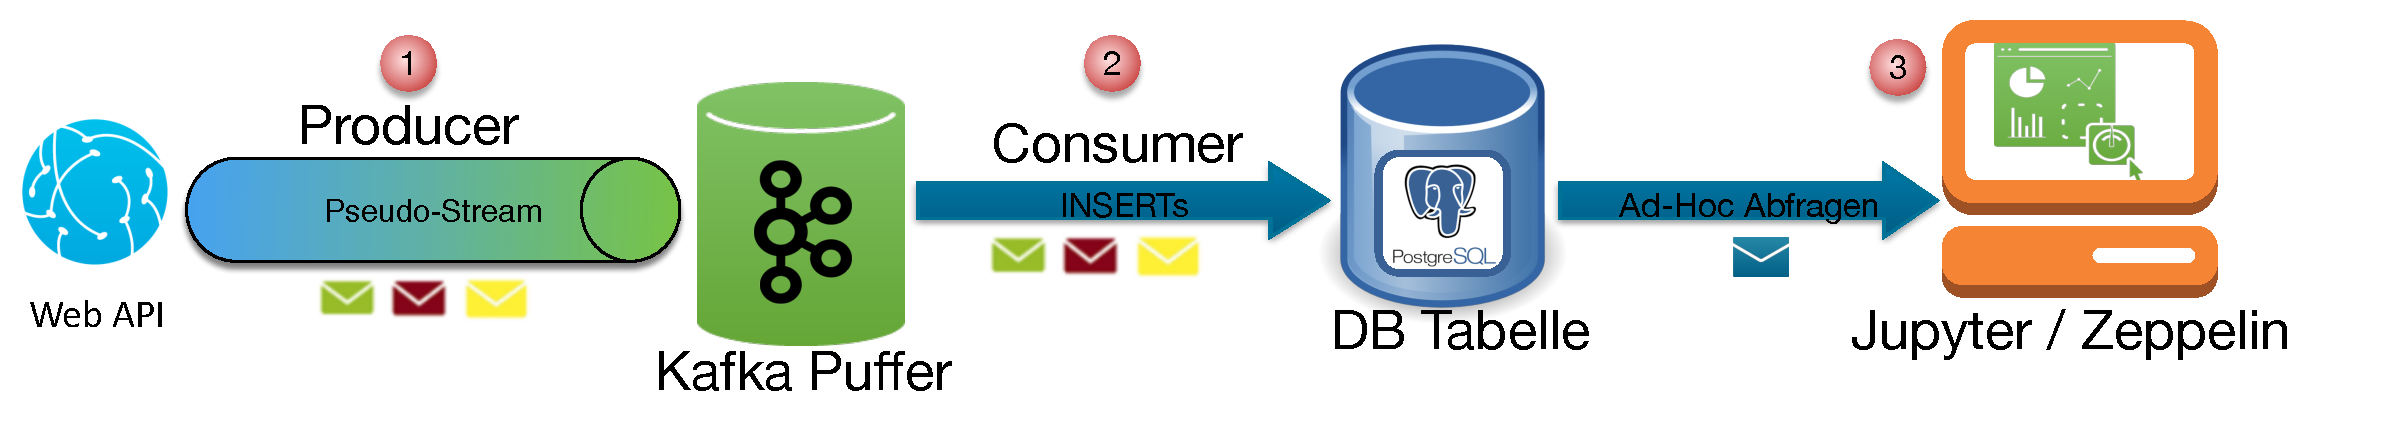
\includegraphics[width=\linewidth]{Overview_kappa.pdf}
	\caption[Finaler Lösungsentwurf nach $\kappa$]{Finaler Lösungsentwurf nach $\kappa$}
	\label{fig:OurKappaArchitecture}
\end{figure}

Schritt \textbf{(1)} bleibt unverändert, wohingegen in Schritt \textbf{(2)} nur noch ein einziger Consumer die Nachrichten des Kafka Topics subskribiert und direkt in eine Datenbanktabelle weiter leitet. Der zweite Consumer sowie Voraggregationen in PostgreSQL entfallen.  Somit muss in den Zeppelin- bzw. Jupyter-Notebooks \textbf{(3)} auf nur eine Datenquelle zugegriffen werden, um die Daten auszuwerten und zu visualisieren.
%Warum Kappa? Daten sind endlich aber ausreichend für unsere Bedürfnisse.Haben eh nur Pseudostream.


%https://www.confluent.io/blog/simplest-useful-kafka-connect-data-pipeline-world-thereabouts-part-1/
